% flashcards-title: Hundred grid with a shaded block
% flashcards-desc: A large square divided into a ten-by-ten grid of one hundred equal small squares. A solid block of small squares beginning at the top left is shaded; the remaining squares are white.
\documentclass[tikz]{standalone}
\usetikzlibrary{arrows.meta,patterns}

\definecolor{qraNavy}{HTML}{17324D}
\definecolor{qraBlue}{HTML}{2B6CB0}
\definecolor{qraGold}{HTML}{B7791F}
\definecolor{qraPale}{HTML}{EAF2F8}
\definecolor{qraGray}{HTML}{5C6773}

\tikzset{
  qra axis/.style={draw=qraNavy, line width=1.2pt},
  qra tick/.style={draw=qraNavy, line width=1pt},
  qra guide/.style={draw=qraGray, densely dashed, line width=0.8pt},
  qra counter/.style={circle, draw=qraNavy, fill=qraPale, line width=0.9pt, minimum size=7mm, inner sep=0pt},
  qra label/.style={font=\sffamily\bfseries, text=qraNavy},
  qra small label/.style={font=\sffamily, text=qraNavy},
}

\begin{document}
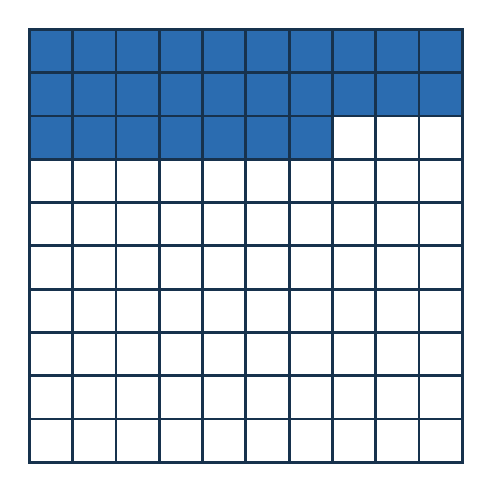
\begin{tikzpicture}[x=0.55cm,y=0.55cm]
  % Shaded block: two full top rows plus seven squares of the third row
  \foreach \c in {0,...,9} \fill[qraBlue] (\c,9) rectangle ++(1,1);
  \foreach \c in {0,...,9} \fill[qraBlue] (\c,8) rectangle ++(1,1);
  \foreach \c in {0,...,6} \fill[qraBlue] (\c,7) rectangle ++(1,1);
  % Grid lines over the fills
  \foreach \i in {0,...,10} {
    \draw[qra tick] (\i,0) -- (\i,10);
    \draw[qra tick] (0,\i) -- (10,\i);
  }
  \draw[qra axis] (0,0) rectangle (10,10);
\end{tikzpicture}
\end{document}
